\documentclass[varwidth=true, border=2pt]{standalone}
\usepackage{tikz}
\usetikzlibrary{calc,shadings}
\usepackage{pgfplots}

\begin{document}
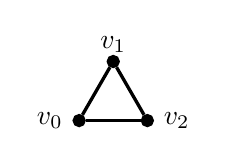
\begin{tikzpicture}[scale=0.5]
    \tikzstyle{point}=[circle,thick,draw=black,fill=black,inner sep=0pt,minimum width=4pt,minimum height=4pt]
    \node (a)[point,label={[label distance=0cm]180:$v_0$}] at (210:1cm) {};
    \node (b)[point,label={[label distance=0cm]0:$v_2$}] at (330:1cm) {};
    \node (c)[point,label={[label distance=-0.1cm]90:$v_1$}] at (90:1cm) {};

    \draw[very thick] (a) edge node  {} (b);
    \draw[very thick] (b) edge node  {} (c);
    \draw[very thick] (c) edge node  {} (a);
\end{tikzpicture}
%\newcommand{\triangleSimplizialkomplex}{\mathord{\includegraphics[height=5ex]{triangle.pdf}}}
%Es gilt $x=\triangleSimplizialkomplex$ und
\end{document}
